\documentclass[a4paper, 12pt]{article}
\usepackage{amsmath, amssymb}

\usepackage[finnish]{babel}
\usepackage[utf8x]{inputenc}
\usepackage{fancyhdr}
\usepackage{listings}


\usepackage{listings}
\usepackage{color}

\usepackage{graphicx}
\usepackage{hyperref}
\usepackage{wrapfig}
\usepackage{lscape}
\usepackage{rotating}
\usepackage{epstopdf}


\lstset{ %
  backgroundcolor=\color{white},
  basicstyle=\footnotesize,
  language=Java,
  tabsize=2
}

\rhead[R]{Alexey Sofiev \\ \texttt{013573003}}
\chead[C]{\Large AOL 1-2, tiiviskurssi, laskari 3}
\title{AOL laskarit I}
\begin{document}
\renewcommand{\headrulewidth}{0pt}
\setlength{\headheight}{30pt}
\pagestyle{fancy}

\section*{Tehtävä 1}

Edellisen työselostuksen perusteella todetaan tunnetuksi, että:

\begin{equation}
ln (x+\triangle x) \approx ln(x) + \frac{\sigma_x}{x}
\label{eq:lnVirhe}
\end{equation}

Näin olleen kun tiedetään että massalla m on vakiotarkkuus $\sigma_m $ (1g), niin ln m on Kaavan \ref{eq:lnVirhe} perusteella 
\begin{equation}
Tarkkuus\ ln(m)\ on\ \frac{\sigma_m}{m} \longrightarrow^{sijoitus\ 1g} = \frac{\textbf{1g}}{\textbf{m}}
\end{equation}

Ja sitten ln v on samalla tavalla:

\begin{equation}
Tarkkuus\ ln(v)\ on\ \frac{\sigma_v}{v} 
\stackrel{sijoitus}{\longrightarrow} \textbf{0.05}
\end{equation}

% Kartion ilmavastuskerroin 0.5

\section*{Tehtävä 2}
Tehtäväannosta tiedetään että putoavalle kartiolle pätee:
\begin{equation}
mg=\gamma v^n
\label{eq:BasicEquation}
\end{equation}
Jossa m on kartion massa (muuttuja), g putoamiskiihtyvyys maan pinnalla (vakio, 9.81 $m/s^2$), $\gamma$ on ilmanvastuskerroin (vakio, 0.5 kartiolle), v on rajanopeus (muuttuja), ja n on reaaliluku jota määritetään.

Tämän riippuvuuden voidaan kirjoittaa muotoon:

\begin{equation}
ln(m)= ln \left( \frac{\gamma}{g} \right)+ n\ ln(v)
\label{eq:LogEquation}
\end{equation}
 
Kaavan \ref{eq:BasicEquation} perusteella saadaan:

\begin{equation}
v=\sqrt[n]{\frac{mg}{\gamma}}
\label{eq:vEquation}
\end{equation}

Saatua Kaava \ref{eq:vEquation} käytetään tässä tehtävässä v:n arvojen laskemiseksi.

Edellisestä tehtävästä tunnetaan epätarkkuudet, joten saadaan

\begin{sidewaysfigure}[!hbt]
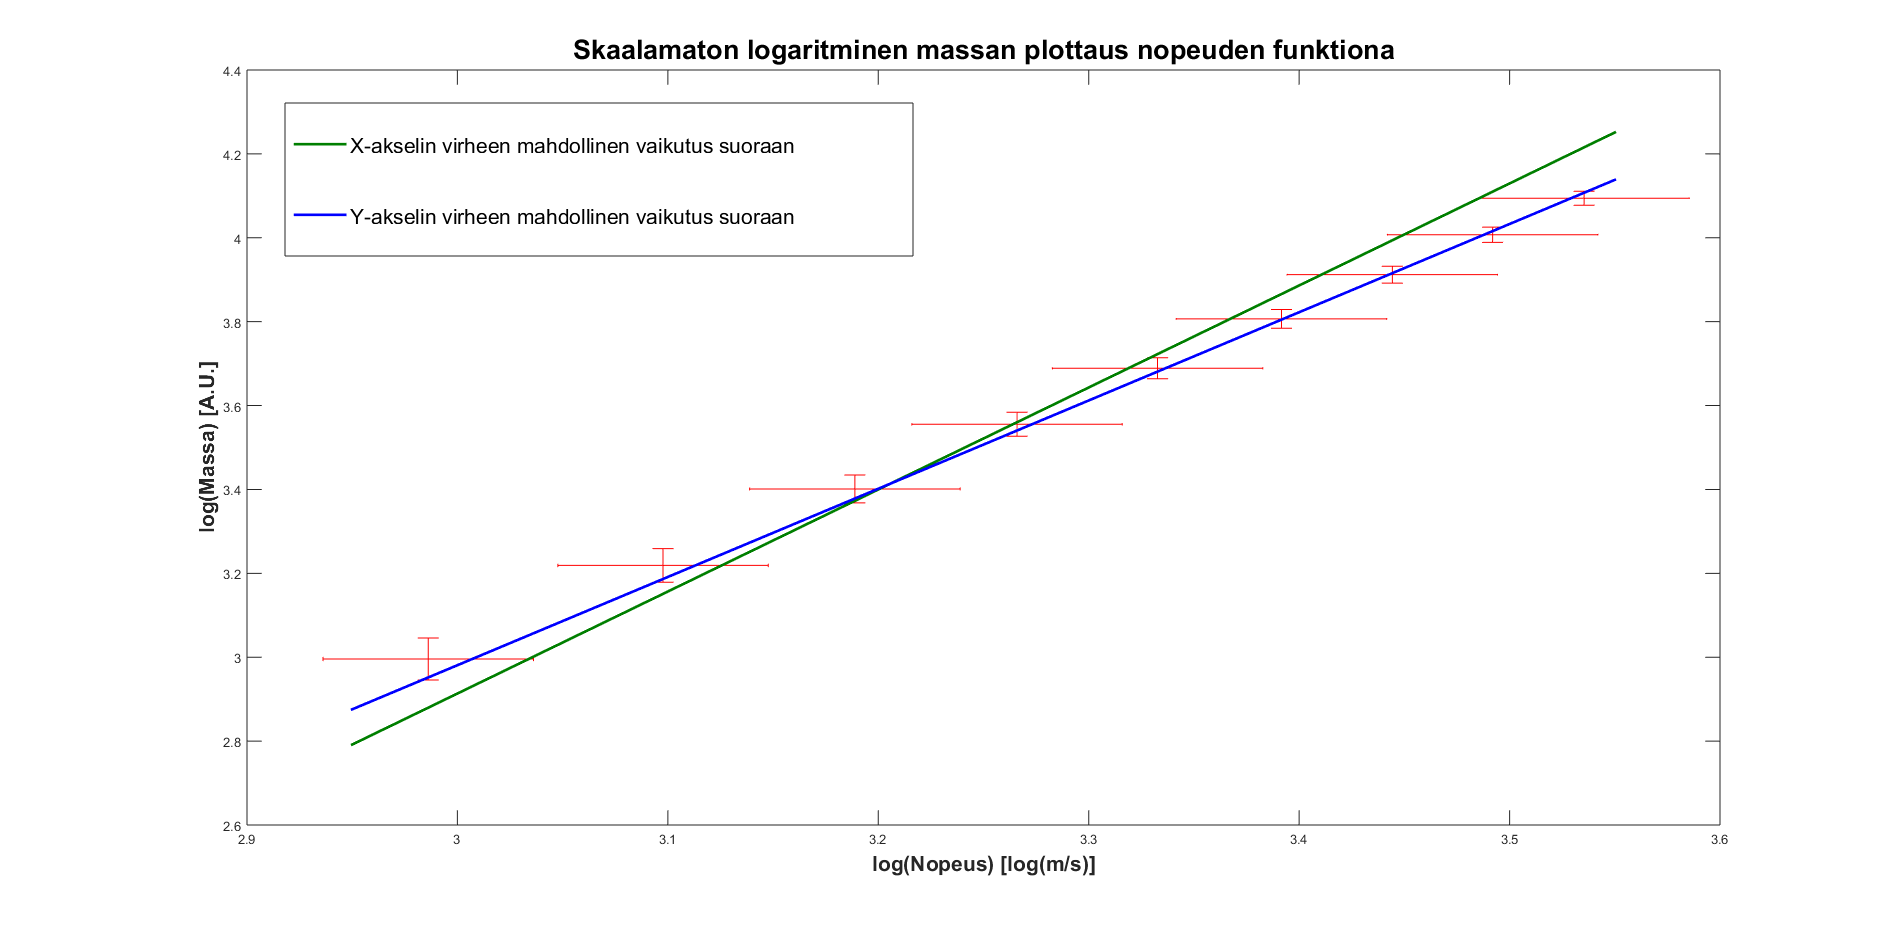
\includegraphics[width=0.99\textwidth]{Laskari3_AOL/teht2_1652}
\caption{Tehtävän 2 kuvaaja, joka esittää massan ja nopeuksien logaritmista riippuvuutta virhepalkineen. Punaisena mittauspisteet ja molempien akselien virhepalkit, sinisena y-akselien poikkeaman mukaan sovitettu suora ja vihreänä x-akselin mukainen.}
\label{fig:teht2Im}
\end{sidewaysfigure}

Kuvasta \ref{fig:teht2Im} nähdään että \textbf{y-akselin vaikutus on huomattavasti pienempi kuin x-akselin vaikutus kulmakertoimeen.
}


\section*{Tehtävä 3}
Suoran sovitus monisteesta sivulta 14 lasketaan apusuure D:

\begin{equation}
D= \sum_i \frac{1}{\sigma_i} \sum_i \frac{x_i^2}{\sigma_i^2}- \left(\sum_i \frac{x_i}{\sigma_i^2} \right)^2
\label{eq:apusuureD}
\end{equation}
jossa $x_i$ on datasarja, ja $\sigma$ on epätarkkuus alaviitteen suhteen.


Kaavaa \ref{eq:apusuureD} hyödyntäen saadaan suoran kulmakertoimen virhe, joka on

\begin{equation}
\sigma_{kulmakerroin}^2 = \frac{1}{D} \sum_i \frac{1}{\sigma_i}
\label{eq:sigmaN}
\end{equation}

Käyttäen kaavaa \ref{eq:sigmaN} saadaan tarkkuudeksi mikäli m on 10 g välein 20 -- 60:

\begin{equation}
\sigma_n /n = \textbf{1.661*10}^{\textbf{-8}}
\label{eq:tarkkuus}
\end{equation}

\section*{Tehtävä 4}

Hyödyntäen Kaavan \ref{eq:tarkkuus} antamaa lauseketta toistetaan lauseke kun m on 5, 10 ja 20 g välein.

Saadaan tuloksiksi:

\begin{equation}
\frac{\sigma_{n,5g}}{ n_{(=9)}}  = 2.647* 10^{-5}
\end{equation}
\begin{equation}
\frac{\sigma_{n,10g}}{ n_{(=5)}}  = 5.764* 10^{-5}
\end{equation}
\begin{equation}
\frac{\sigma_{n,20g}}{ n_{(=3)}}  = 1.061* 10^{-4}
% D =
% 
%    3.9652e+05
% 
% 
% sigmaN =
% 
%    5.6744e-08
% 
% 
% D =
% 
%    1.5052e+05
% 
% 
% sigmaN =
% 
%    8.3046e-08
% 
% 
% D =
% 
%    7.4072e+04
% 
% 
% sigmaN =
% 
%    1.0125e-07
\end{equation}

Näistä nähdään että \textbf{paras tarkkuus saavutetaan kun mitataan 10 g välein.}

\textbf{Huomautus:} Koodit tehtävään 4 ovat teht3.m :ssa, kun Tehtävä 3 on vain yksi osatapaus 4. tehtävästä. 

\section*{Analysointikoodi}
\url{https://github.com/AleksDark/TiivisLabrat/tree/master/Laskarit/Laskari3/Laskari3_AOL}

%\section*{Viitteet}
\begin{thebibliography}{1}

\bibitem{Tyoohje}
  AOL 1-2 Työohje,
  Helsingin yliopisto,
  2016.

\bibitem{Suoran sovitus}
  AOL 1-2, Työphje,
  \emph{Kirjallisuus: Suoran sovitus},
  \url{https://moodle.helsinki.fi/pluginfile.php/1228496/mod_resource/content/2/pns_sovitus.pdf}
  2016.


%\bibitem{lamport94}
%  Leslie Lamport,
%  \emph{\LaTeX: a document preparation system},
%  Addison Wesley, Massachusetts,
%  2nd edition,
%  1994.

\end{thebibliography}



\iffalse

\begin{sidewaysfigure}[!hbt]
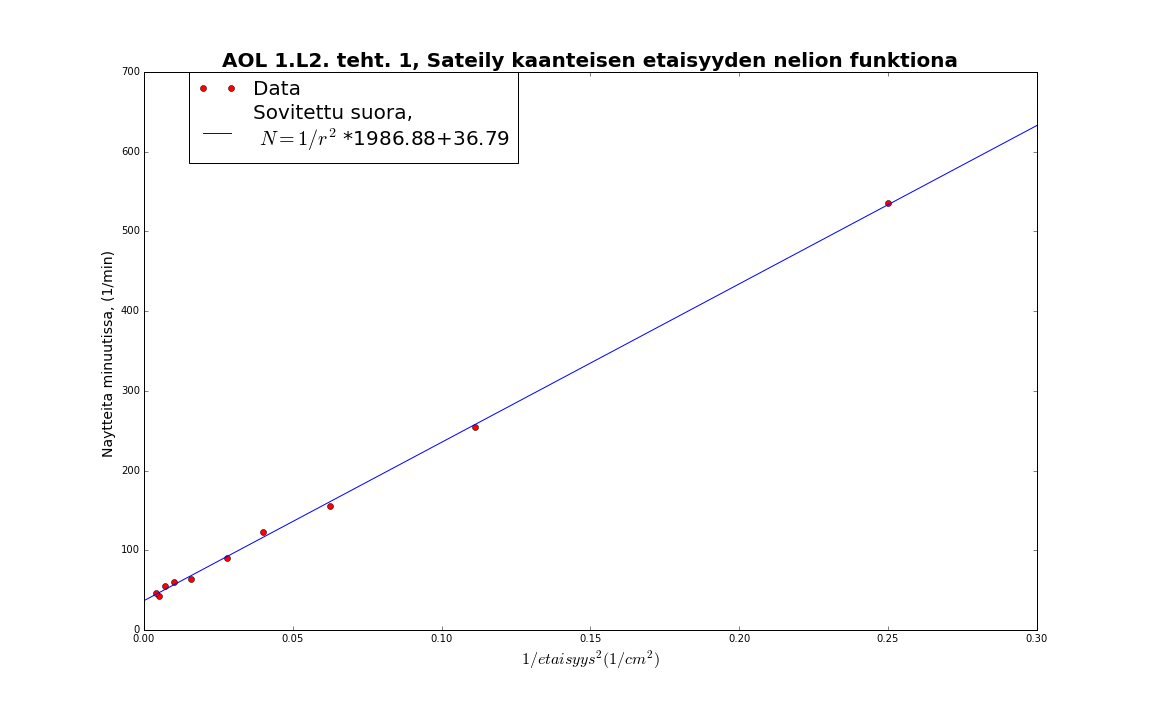
\includegraphics[width=0.99\textwidth]{1}
\caption{Tehtävä 1:n tulos, (1/$r^2$, N)- kuvaajassa esitetty datajoukko ja sovitettu suora ilman painokertoimia.}
\end{sidewaysfigure}

Iso / Paremman laatuinen / alkuperäinen: \url{"https://github.com/AleksDark/TiivisLabrat/blob/master/Laskarit/Laskari2/1.png}

Esitetyssä kuvassa punaiset pisteet ovat annettu datajoukko ja  sininen on siihen sovitettu yhtälö.



\section*{Tehtävä 2}
\begin{sidewaysfigure}[!hbt]
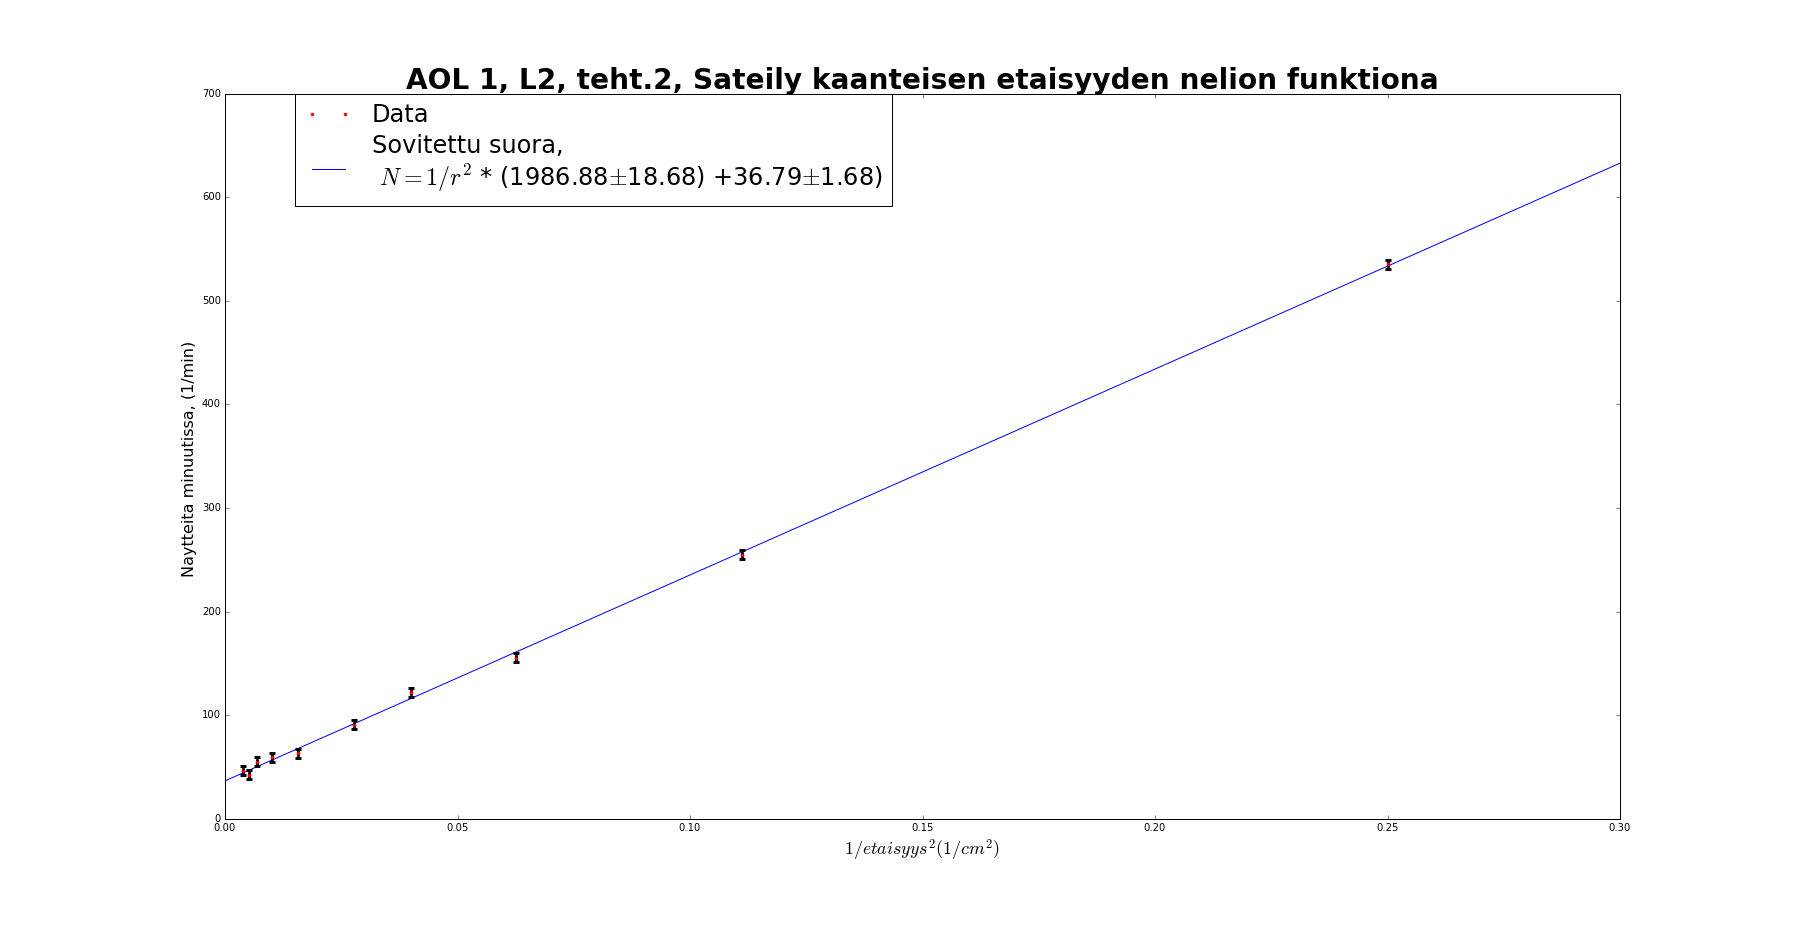
\includegraphics[width=1\textwidth]{2}
\caption{Tehtävä 2:n tulos, (1/$r^2$, N)- kuvaajassa esitetty datajoukko ja sovitettu suora hyödyntäen $\chi^2$ jakaumaa datalle.}
\end{sidewaysfigure}

Iso / Paremman laatuinen / alkuperäinen: \url{"https://github.com/AleksDark/TiivisLabrat/blob/master/Laskarit/Laskari2/2.png}

Esitetyssä Kuva 2:ssa punaiset pisteet ovat annettu datajoukko ja  sininen on siihen sovitettu yhtälö. Virhepalkit ovat mustana, sekä pieniä.

Epätarkkuudet ja sovitukset ovat tehty hyödyntäen Moodle AOL1-2, Suoran sovitusmonistetta.

Saadut arvot ovat:\\
Suoran sovitusparametrit:  [ 1986.88499301    36.79466127]\\
D:  0.00154369042952 \\
Epätarkkuudet: 18.684 ja 1.687

\section*{Tehtävä 3}
\begin{sidewaysfigure}[!hbt]
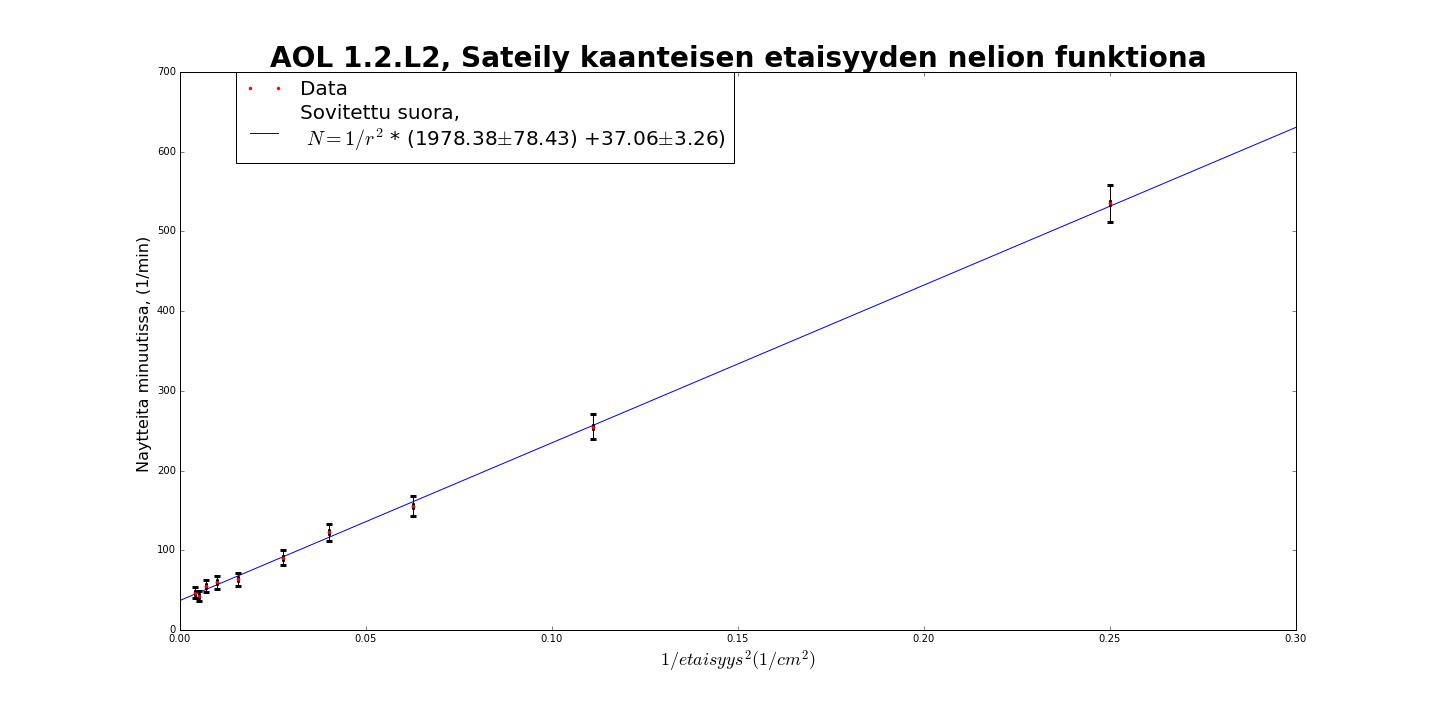
\includegraphics[width=1\textwidth]{3}
\caption{Tehtävä 3:n tulos, (1/$r^2$, N)- kuvaajassa esitetty datajoukko ja sovitettu suora hyödyntäen tietoa että hajonta on $\sqrt{N}$.}
\end{sidewaysfigure}

Iso / Paremman laatuinen / alkuperäinen: \url{"https://github.com/AleksDark/TiivisLabrat/blob/master/Laskarit/Laskari2/3.png}\\

Parametrit suoran sovitukseen:  [ 1978.388    37.063]\\
D : 2.06090577671e-05\\
Epätarkkuudet:  78.432 ja 3.261


\paragraph{Johtopäätökset}
Huomataan hieman erilaiset parametrit tehtävä 2 vs 3 ja erilaiset epätarkkuudet. Tehtävässä 2 jotkut pisteet jäävät virhepalkineen suoran sovituksen ulkopuolelle, puolestaan teht 3 sovituksessa kaikki pisteet ovat virherajojen puutteessa sisällä.

\section*{Tehtävä I}
\subsection*{a)}
Parittomat luvut voidaan ilmaista muodossa $k=2n+1$
\begin{center}
\begin{eqnarray*}
&& \left(2n+1\right)^2-1 \\ 
& = & 4n^2+4n+1-1 \\
& = & 4n^2+4n \\
& = & 4\left(n^2+n\right)
\end{eqnarray*}
\end{center}
Kaikki luvut ovat jaollisia neljällä, siten myös parillisia.
\subsection*{b)}
Luvut, jotka eivät ole kolmella jaollisia, voidaan ilmaista muodossa $k=3n+1$

\begin{center}
\begin{eqnarray*}
&& \left(3n+1\right)^2-1 \\
& = & 9n^2+6n+1-1 \\
& = & 3\left(3n^2+2n\right)
\end{eqnarray*}
\end{center}
Eli kaikki luvut ovat jaollisia kolmella.
\subsection*{c)}
Voidaan merkitä $a=b=c$
\begin{center}
\begin{eqnarray*}
a\left(b+c\right)&<&a+b+c \\
a\left(a+a\right)&<&a+a+a \\
2a^2 &<& 3a
\end{eqnarray*}
\end{center}
Tehdään sijoitus $a=1$.

\begin{center}
\begin{eqnarray*}
2 \times 1^{2} &<&  3 \times 1 \\
2 &<& 3
\end{eqnarray*}
\end{center}
Väite on tosi. Eli $a\left(b+c\right)<a+b+c$ pätee joillain arvoilla $a,b,c \in \mathbb{N}$
\subsection*{d)}
Edellisen kohdan perusteella saadaan $2a^2<3a$. Tehdään sijoitus $a=2$.
\begin{center}
\begin{eqnarray*}
2 \times 2^2 &<& 3 \times 2 \\
8 &<& 6
\end{eqnarray*}
\end{center}
Väite \emph{millä tahansa kolmella luvulla $a,b,c \in \mathbb{N}$   $a\left(b+c\right)<a+b+c$} ei tämän ristiriidan takia voi pitää paikkansa, sillä on olemassa jokin luku, joka kuuluu luonnollisten lukujen joukkoon, joka ei toteuta anntettua väitettä.

\section*{Tehtävä II}
\subsection*{a)}
\texttt{!A \&\& !B} ja \texttt{!(A \&\& B)} ovat yhtäsuuret. \\
\texttt{!A || !B} ja \texttt{!(A || B)} ovat yhtäsuuret.
\subsection*{b)}
\texttt{!(!A || !B) \&\& B} $\Rightarrow$ \texttt{A \&\& B}
\subsection*{c)}
\texttt{(A || !B) \&\& (B || !A)} $\Rightarrow$ \texttt{(A \&\& B) || (!A \&\& !B)}
\subsection*{d)}
\texttt{!(((A || !A) || A || B) \&\& !A)} $\Rightarrow$ \texttt{A}

\section*{Tehtävä III}
\subsection*{a)}
$\_{2}128$ \\
$128/\underbrace{2/2/2/2/2/2/2}_\text{7}=1$ \\
$\log_{2}128=7$
\subsection*{b)}
$log_{4}4 \\
4/\underbrace{4}_\text{1}\\
log_{4}4=1$
\subsection*{c)}
$log_{3} 81 \\
81/\underbrace{3/3/3/3}_{4}=1 \\
log_{3}81=1
$
\subsection*{d)}
$log_{11}1$\\
Koska $log_{n}a=x \Leftrightarrow n^{x}=a$ ja $x^{0}=1$, on vastaus $0$.
\subsection*{e)}
$log_{11}121\\
121\underbrace{/11/11}_{2}=1$
\subsection*{f)}
$log_{10}100000\\
100000/10^{5}=1\\
log_{10}100000=5$
\subsection*{g)}
$log_{2}2^{19}\\
2^{19}/2^{19}=1\\
log_{2}2^{19}=19$

\section*{Tehtävä VI}
\subsection*{a)}
Suurin mahdollinen luku on juuri ennen \emph{roll-overia}, eli $2^{7}-1=1 \times 2^6 +1 \times 2^5 +1 \times 2^4 +1 \times 2^3 +1 \times 2^2 +1 \times 2^1 +1 \times 2^0 +=127$
$2^{7}-1$, sillä se potenssinumerointi alkaa nollasta.
\subsection*{b)}
Edellisen logiikan mukaan suurin mahdollinen tasan yhdeksän merkin mittainen binääriluku on $2^9-1=511$\\
Pienin puolestaan on joko $000000000_2$, mutta mikäli sen täytyy alkaa merkitsevällä luvulla (eli alusta ei voida karsia mitään pois), niin saadaan $100000000_2=256$
\subsection*{c)}
Luku $100111010110100110111_2$ on pariton, sillä ainoa paikka, mistä pariton luku binääriesityksestä saadaan, on kauimmainen symboli oikealla, ennen desimaalipilkkua, sillä $2^0=1$ on ainoa tapa saada pariton luku binäärijärjestelmään.
\subsection*{d)}
$400_{10}$ on binäärijärjestelmässä $9$-merkkiä pitkä, sillä luku on pienempi kuin $2^9=512$, mutta suurempi kuin $2^8=256$. Binääriesityksenä $400_{10}$ on $110010000_2$
\subsection*{e)}
Yleinen funktio binäärisen esityksen pituudelle: \\
$f(x) = \left\{
   \begin{array}{l l}
    1 & x = 0 \\
    \lfloor log_2 x\rfloor +1 & x \neq 0
  \end{array} \right.
$
\section*{Tehtävä V}
\subsection*{a)}
\begin{lstlisting}
public class Rekursiivisuus {
    public static void main(String[] args) {
        rekurs(3);
    }
    public static void rekurs(int k) {
        tahti(k);
        System.out.println("");
        if (k > 0) rekurs(k - 1);
    }
   public static void tahti(int j) {
        if (j > 0) tahti(j-1);   
        System.out.print("*");
    }
}
\end{lstlisting}
\subsection*{b)}
\begin{lstlisting}
public class Rekursiivisuus {
    public static void main(String[] args) {
        rekurs(3);
    }
     public static void rekurs(int k) {
        if (k > 0) rekurs(k - 1);
        tahti(k);
        System.out.println("");
    }

   public static void tahti(int j) {
        if (j > 0) tahti(j-1);   
        System.out.print("*");
    }
}
\end{lstlisting}
\newpage
\subsection*{c)}
\begin{lstlisting}
public class Rekursiivisuus {
    public static void main(String[] args) {
        rekurs(3);
    }
    public static void rekurs(int k) {
        if (k > 0) {
            rekurs(k - 1);
            tahti(k);
            System.out.println("");
            rekurs(k - 1);
        }
    }
    public static void tahti(int j) {
        if (j > 0) {
            tahti(j - 1);
            System.out.print("*");
        }
    }
}
\end{lstlisting}
\subsection*{d)}
\begin{lstlisting}
public class Rekursiivisuus {
    static int n;
    public static void main(String[] args) {
        n=1;
        rekurs(3);
        }
    public static void rekurs(int k) {
        if (k > 0) {
            int monesko = n;
            n++;
            rekurs(k - 1);
            tahti(k);
            System.out.println(" "+monesko);
            rekurs(k - 1);
        }
    }
    public static void tahti(int j) {
        if (j > 0) {
            tahti(j-1);
            System.out.print("*");
        }
    }
}
\end{lstlisting}
\newpage
\section*{Tehtävä VI}
\subsection*{a)}
\begin{lstlisting}
public class Rekursiivisuus {
    static int k=0;
    public static void main(String[] args) {
        System.out.println(rekurs(4, 7));
        }
    public static int rekurs(int i, int j) {
        if (i==0 || j==0) return 0;
        k+=j;
        if (i==1) return k;
        return rekurs(i-1, j);
    }
}
\end{lstlisting}

\fi
\end{document}
